% oocriterion.tex
\documentclass[main.tex]{subfiles}
\begin{document}
\chapter{A Novel Failure Criterion} \label{ch:oocrit}
\epigraph{\textit{The Osswald$^2$ criterion}}

As described during Section \ref{sec:FC} of Chapter \ref{ch:bg}, currently available Failure Criteria fail to completely integrate interaction effects into the modeled failure behavior of anisotropic materials. In 2017, Paul and Tim Osswald proposed a model that attempts to overcome these limitiations \cite{Osswald2017a}. This recent failure criterion has the following characteristics:
\begin{itemize}
	\item \textbf{Tensor based and purely mathematical}: as opposed to phenomenological or mechanistic models such as the Puck or Cuntze failure criteria.
	\item \textbf{Based on the Gol'denblat-Kopnov model}.
	\item \textbf{Includes stress interactions that other models neglect}.
\end{itemize}

Originally titled \textquotedblleft A Strength Tensor Based Failure Criterion with Stress Interactions\textquotedblright, it will be referred in this work as the Osswald-Osswald Criterion (OOC). This chapter will describe the Gol'denblat-Kopnov model upon which the OOC is based, followed by a proper description of how this novel model implements stress interactions.

\section{The Gol'denblat-Kopnov Model}\label{sec:GKC}
The Gol'denblat-Kopnov Criterion (GKC) describes a mathematical function that depends on the stress state of an anisotropic material. Should the computation of this expression exceed a threshold, part failure is to be expected. To that end, a scalar function that depends on stress tensors that completely characterize the state of the material was developed \cite{Goldenblat1965}. This function is shown in Equation \ref{eq:GKCgen}, where stresses are denoted $\sigma$.

\begin{equation} \label{eq:GKCgen}
f=(F_{ij}\sigma_{ij})^\alpha + (F_{ijkl}\sigma_{ij}\sigma_{kl})^\beta + (F_{ijklmn}\sigma_{ij}\sigma_{kl}\sigma_{mn})^\gamma + ...
\end{equation}

The terms $F_{ij}$, $F_{ijkl}$ and $F_{ijklmn}$ represent second, fourth and sixth order tensors respectively. These terms of the equation depend on engineering strength parameters, such as the ultimate tensile and compressive strengths of the material in a particular load direction \cite{Osswald2017a}. Due to the complexity associated with using higher order tensors, Gol'denblat and Kopnov limited their approach to using only the second and fourth order terms. Thus Equation \ref{eq:GKCgen} is reduced to:

\begin{equation} \label{eq:GKCgenTrunc}
f=(F_{ij}\sigma_{ij})^\alpha + (F_{ijkl}\sigma_{ij}\sigma_{kl})^\beta
\end{equation}

In order to attain a linear criterion scalar function, the exponents $\alpha$ and $\beta$ were assigned values of 1 and 1/2 respectively. Finally, in plain stress scenarios, the GKC becomes:

\begin{equation} \label{eq:GKCfinal}
\begin{split}
f=F_{11}\sigma_{11} + F_{22}\sigma_{22} + F_{12}\tau_{12} + (F_{1111}\sigma_{11}^{2} + F_{2222}\sigma_{22}^{2} + F_{1212}\tau_{12}^{2} \\ + 2F_{1122}\sigma_{11}\sigma_{22} + 2F_{1112}\sigma_{11}\tau_{12} + 2F_{2212}\sigma_{22}\tau_{12})^{1/2}
\end{split}
\end{equation}

Note that in Equation \ref{eq:GKCfinal} $\sigma$ and $\tau$ denote normal and shear stresses respectively. Figure \ref{fig:loaddir} depicts an anisotropic material and all the possible loading directions for reference.

\begin{figure}[h]
	\center
	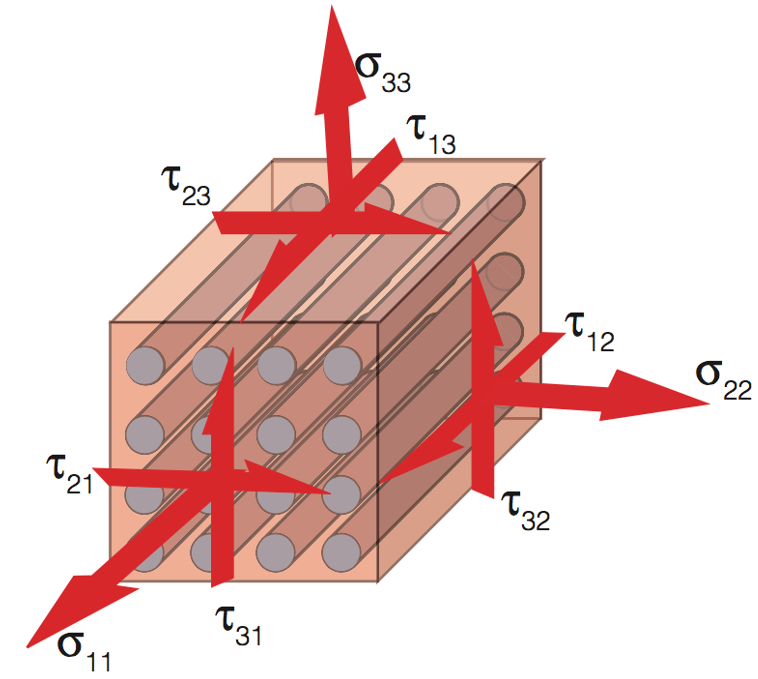
\includegraphics[height=5cm]{reference_cube}
	\caption{Different load directions in an anisotropic material} \label{fig:loaddir}
\end{figure}

Per Gol'denblat and Kopnov's design, should Equation \ref{eq:GKCfinal} be greater or equal to 1, part failure is to be expected. However, to simplify calculations, they deliberately assumed the interaction terms $F_{1112}$ and $F_{2212}$ to be zero. This is an important consideration that will come into play when describing the OOC.

Most of the terms in the GKC are obtained through mechanical testing of coupons under pure uniaxial loads in the 1 or 2 direction, or pure shear in the 1-2 plane \cite{Osswald2017a}. In these scenarios, $f$ will be equal to 1 at failure, and the stress state will be known to the user, allowing some of the unknown tensorial parameters to be easily calculated. Using $F_{11}$ and $F_{1111}$ as examples, the process would be as follows:
\pagebreak
\begin{enumerate}
	\item The tensile and compressive strength in the 1-1 direction would be obtained through mechanical testing. These values are named $X_t$ and $X_c$ respectively.
	\item Under these failure conditions, Equation \ref{eq:GKCfinal} is reduced to the following system of equations:
	\[
	\systeme*{1=F_{11}X_t + (F_{1111}X_t^{2})^{1/2}, 1= -F_{11}X_c + (F_{1111}X_c^{2})^{1/2}}
	\]

	\item $F_{11}$ and $F_{1111}$ can be obtained, yielding $F_{11}=\frac{1}{2}(\frac{1}{X_t}-\frac{1}{X_c})$ and $F_{1111}=\frac{1}{4}(\frac{1}{X_t}+\frac{1}{X_c})^2$.
\end{enumerate}

The only exception to this procedure would be the $F_{1122}$ component, which requires measuring the positive and negative shear strengths of a coupon with reinforcement oriented in 45$^\circ$. These parameters are named $S_{45p}$ and $S_{45n}$ respectively. Table \ref{tab:GKparam} summarizes the nomenclature used for the strength parameters required to completely populate the failure function of the GKC. Table \ref{tab:GKtens} summarizes all the tensorial component calculations.

\begin{table} [h]
	\centering
	\caption{Nomenclature of the GKC parameters}
	\begin{tabular}{ c c }
	\toprule
		\textbf{Parameter} & \textbf{Description} \\ 
		\midrule
		$X_t$ & Tensile strength in the 1-1 direction\\
		$X_c$ & Compressive strength in the 1-1 direction\\
		$Y_t$ & Tensile strength in the 2-2 direction\\
		$Y_c$ & Compressive strength in the 2-2 direction\\
		$S_{45p}$ & Positive shear strength for 45$^\circ$ specimen\\
		$S_{45n}$ & Negative shear strength for 45$^\circ$ specimen\\
		$S$ & Shear strength in the 1-2 plane\\
	\bottomrule
	\end{tabular}
	\label{tab:GKparam}
\end{table}

\begin{table} [h]
	\centering
	\caption{Tensorial components of the GKC}
	\begin{tabular}{ c c } 
	\toprule
		\textbf{Component} & \textbf{Formula} \\
		\midrule
		$F_{11}$ & $\frac{1}{2}(\frac{1}{X_t}-\frac{1}{X_c})$\\ [1ex]
		$F_{1111}$ & $\frac{1}{4}(\frac{1}{X_t}+\frac{1}{X_c})^2$\\ [1ex]
		$F_{22}$ & $\frac{1}{2}(\frac{1}{Y_t}-\frac{1}{Y_c})$\\ [1ex]
		$F_{2222}$ & $\frac{1}{4}(\frac{1}{Y_t}+\frac{1}{Y_c})^2$\\ [1ex]
		$F_{12}$ & 0\\ [1ex]
		$F_{1212}$ & $\frac{1}{S^2}$\\ [1ex]
		$F_{1122}$ & $\frac{1}{8}[(\frac{1}{X_t}+\frac{1}{X_c})^2+(\frac{1}{Y_t}+\frac{1}{Y_c})^2-(\frac{1}{S_{45p}}+\frac{1}{S_{45n}})^2]$\\ [1ex]
		\bottomrule
	\end{tabular}
	\label{tab:GKtens}
\end{table}
\pagebreak

\section{The Osswald-Osswald Criterion}\label{sec:OOC}
One of the assumptions made in the GKC is that the components $F_{1112}$ and $F_{2212}$ in Equation \ref{eq:GKCfinal} are null. While this simplifies the model, it essentially neglects any interactions between axial loads and shear stresses, namely, the $\sigma_{11}$ - $\tau_{12}$ and $\sigma_{22}$ - $\tau_{12}$ interactions. Practically, this causes the failure surface developed through the GKC to under predict shear strengthening effects exhibited by anisotropic materials loaded in combined axial and shear conditions. Figure \ref{fig:GKClimit} shows a comparison between experimental data obtained from the first World Wide Failure Exercise (WWFE-I) and the GKC envelope developed for this material. In this example, a unidirectional glass reinforced epoxy composite was tested in multiple loading conditions in the $\sigma_{22}$ and $\tau_{12}$ stress plane. The resulting data was used to develop a failure envelope following the GKC. Note how on the first quadrant, the model follows the data closely. However, in the second quadrant, the criterion is relatively conservative, failing to capture the strengthening that occurs when loading the material in compression and shear.   

\begin{figure}[h]
	\center
	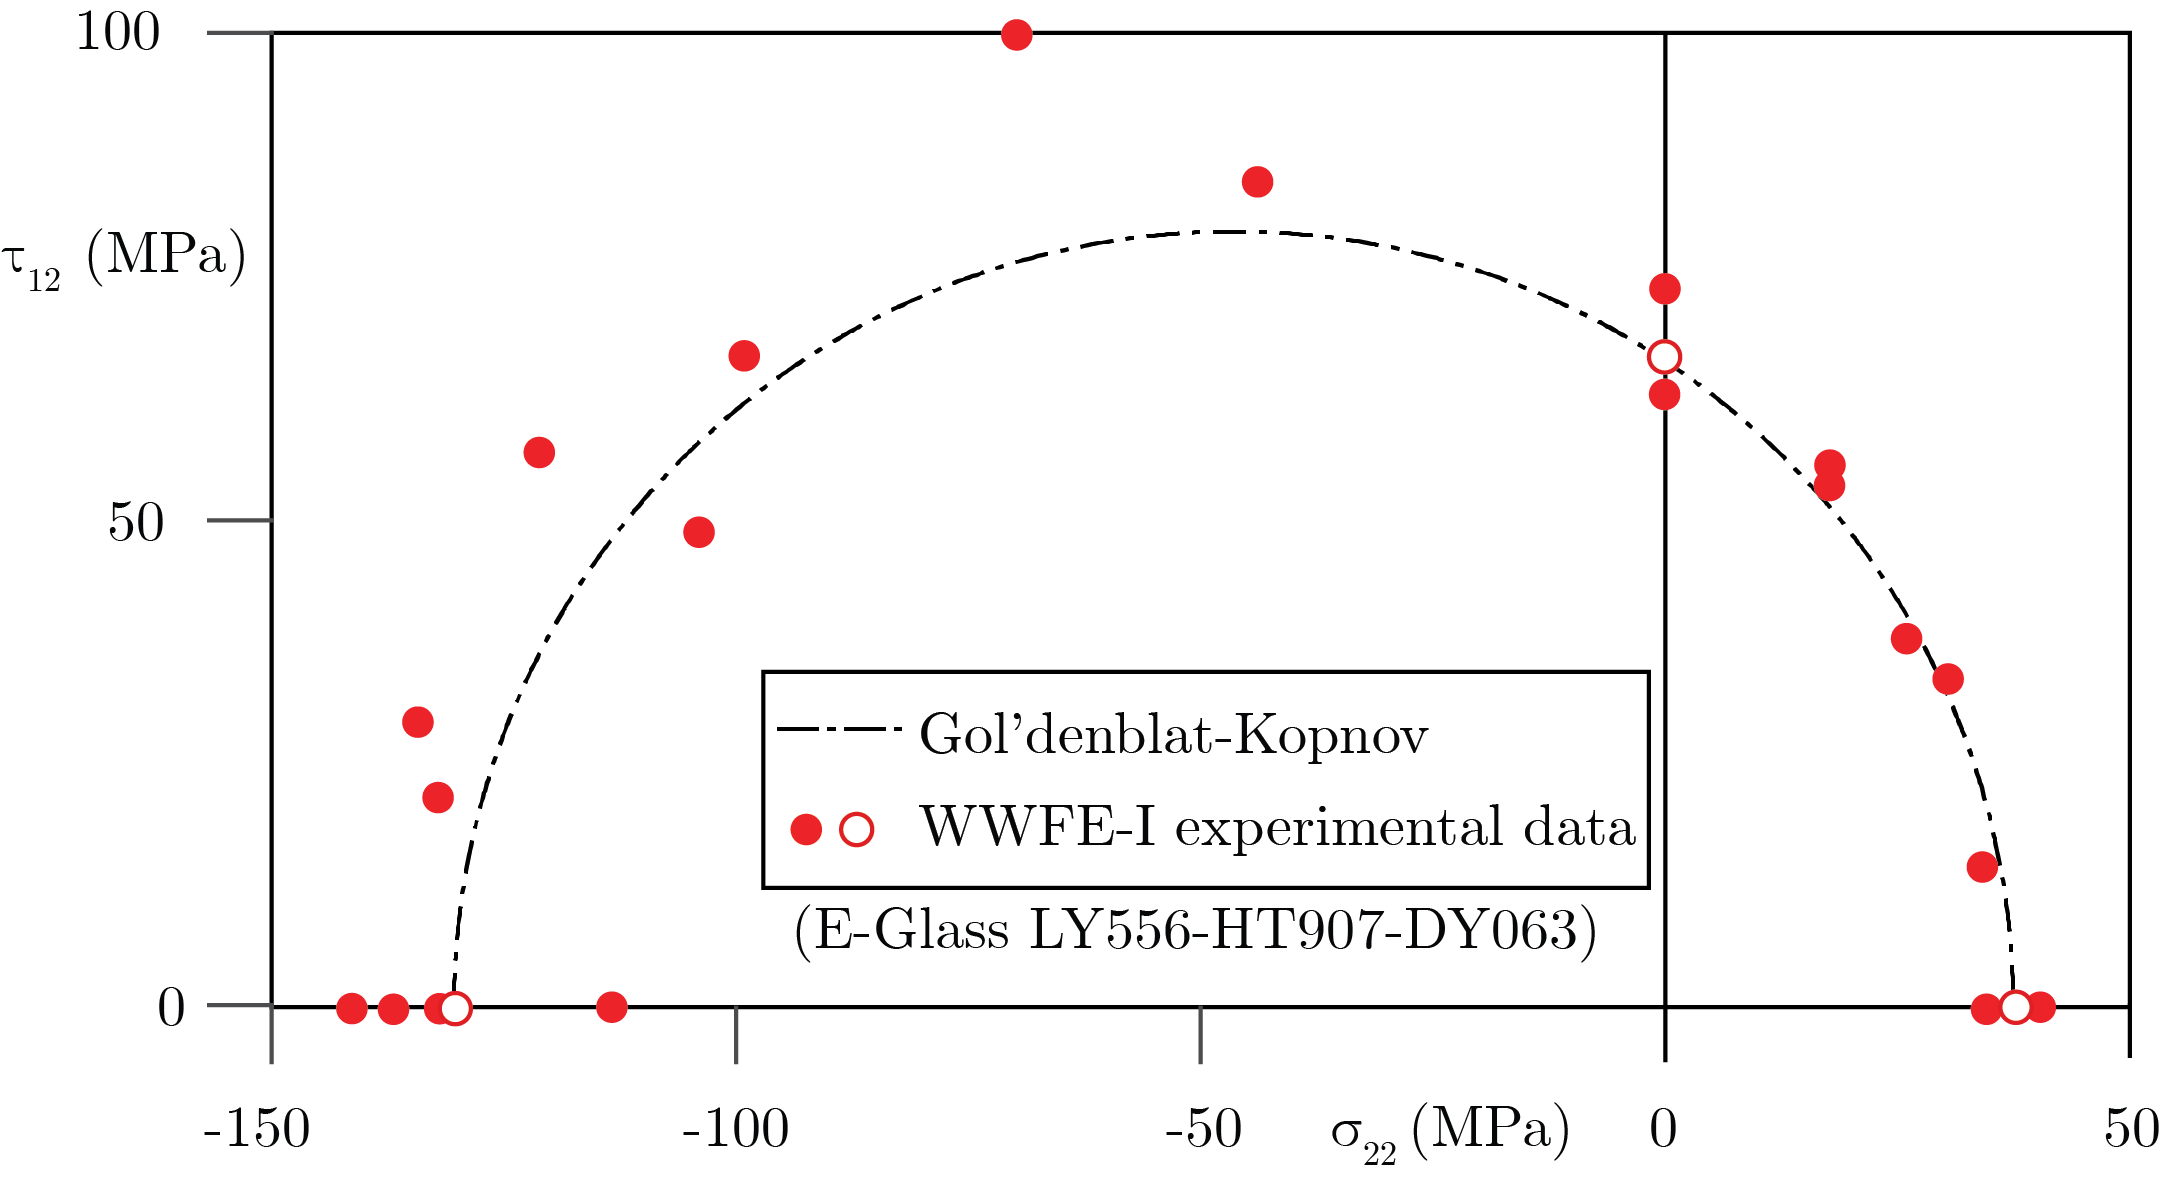
\includegraphics[height=7cm]{GK_thesis}
	\caption{GKC failure surface developed using data from the WWFE-1} \label{fig:GKClimit}
\end{figure}

The Osswald-Osswald Criterion (OOC) attempts to overcome these limitations by building upon the GKC. For the OOC, the interaction effects are captured through the use of the slopes of the failure surface at any of the points where the engineering strength is known within a particular stress plane \cite{Osswald2017a}. In this failure scenario, the stress state of the coupon is known and easy to implement into Equation \ref{eq:GKCfinal}, where $f=1$. The resulting expression can then be derived with respect to one of the stresses, allowing for the interaction components to be calculated. This is better illustrated through an example. Assuming the component of interest is $F_{2212}$, the procedure to calculate it through the OOC would be as follows:

\pagebreak
\begin{enumerate}
	\item Obtain all the tensorial components possible through the GKC.
	\item Using the $\sigma_{22}$\textendash$\tau_{12}$ stress plane, derive Equation \ref{eq:GKCfinal} as a function of $\sigma_{22}$ in the scenario of failure under pure shear ($f=1$). This yields the expression:
	\begin{equation} \label{eq:OOCex1}
	 0= F_{22}+[F_{1212}S(\frac{d\tau_{12}}{d\sigma_{22}})+F_{2212}S]
	\end{equation}
	 where $\frac{d\tau_{12}}{d\sigma_{22}}$  is the slope of the graph at failure under shear. This term is named $\mu^{2212}$ in the OOC and can be obtained by performing combined loading tests. Refer to Figure \ref{fig:OOCdemo} for a visual representation.
	\item Rearranging Equation \ref{eq:OOCex1} to solve for the unknown $F_{2212}$ gives the following expression:
	\begin{equation} \label{eq:OOCex2}
	F_{2212}=-\frac{F_{22}}{S}-F_{1212}\mu^{2212}
	\end{equation}
\end{enumerate}

\begin{figure}[h]
	\center
	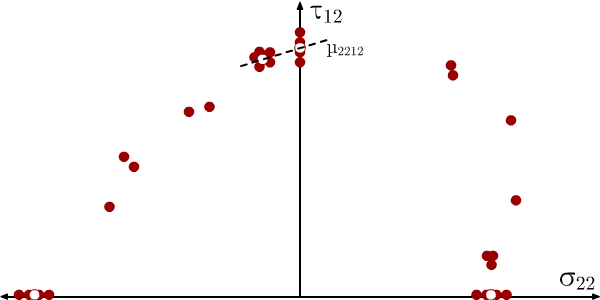
\includegraphics[height=5cm]{OOC_demo_thesis}
	\caption{$\mu^{2212}$ parameter in the $\tau_{12}$ - $\sigma_{22}$ plane} \label{fig:OOCdemo}
\end{figure}

A similar procedure can be followed for any $\sigma_{ii}$-$\tau_{ij}$ interaction, or even any $\sigma_{ii}$-$\sigma_{jj}$ components. For this last scenario, the user has four potential choices of slopes to determine the tensorial component of interest. In the OOC, any slope obtained from a $\sigma_{ii}$-$\sigma_{jj}$ stress plane is named $\lambda^{iijj}$, as opposed to $\mu^{iiij}$ for slopes in a $\sigma_{ii}$-$\tau_{ij}$ reference. A schematic of all possible $\lambda^{iijj}$ is shown in Figure \ref{fig:OOCdemo2}, while Table \ref{tab:OOCcomp} summarizes all the possible interaction factors available through the OOC, where $\tau_{ij}^u$ denotes ultimate shear strength in a particular shear plane. 

\begin{figure}[h]
	\center
	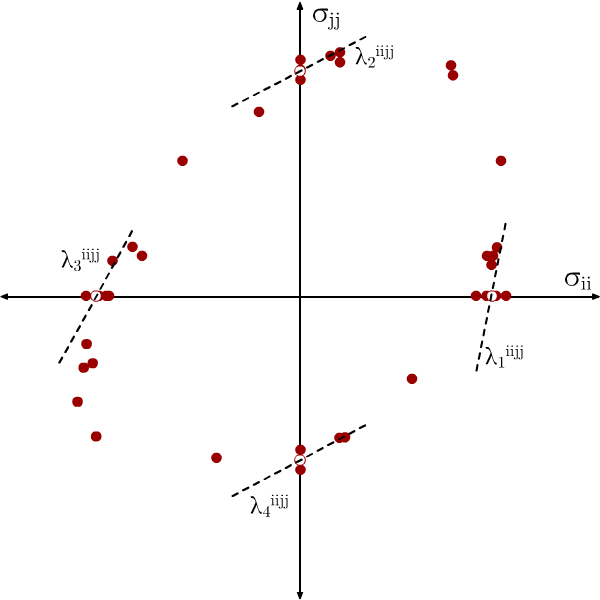
\includegraphics[height=10cm]{OOC_demo_thesis2}
	\caption{$\lambda^{iijj}$ parameters in a generic $\sigma_{ii}$ - $\sigma_{jj}$ stress plane} \label{fig:OOCdemo2}
\end{figure}

\begin{table} [h]
	\renewcommand{\arraystretch}{1.5}
	\centering
	\caption{Interaction components attainable through the OOC}
	\begin{tabular}{ c c } 
		\toprule
		\textbf{Component} & \textbf{Formula} \\
		\midrule
		$F_{iiij}$ & $-\frac{F_{ii}}{\tau_{ij}^u}-F_{ijij}\mu^{iiij}$\\
		$F_{iijj}$ through $\lambda^{iijj}_1$ & $-\frac{(F_{ii}+F_{jj}\lambda^{iijj}_1)F_{iiii}^{1/2}+F_{iiii}}{\lambda^{iijj}_1}$\\
		$F_{iijj}$ through $\lambda^{iijj}_2$ & $-(F_{ii}+F_{jj}\lambda^{iijj}_2)F_{jjjj}^{1/2}-F_{jjjj}\lambda^{iijj}_2$\\
		$F_{iijj}$ through $\lambda^{iijj}_3$ & $\frac{(F_{ii}+F_{jj}\lambda^{iijj}_3)F_{iiii}^{1/2}-F_{iiii}}{\lambda^{iijj}_3}$\\
		$F_{iijj}$ through $\lambda^{iijj}_4$ & $(F_{ii}+F_{jj}\lambda^{iijj}_4)F_{jjjj}^{1/2}-F_{jjjj}\lambda^{iijj}_4$\\
		\bottomrule
	\end{tabular}
	\label{tab:OOCcomp}
\end{table}
\pagebreak
% Nomenclature introduced in this chapter:
\nomenclature[A]{OOC}{Osswald-Osswald Criterion}% 
\nomenclature[A]{GKC}{Gol'denblat-Kopnov Criterion}% 

% Symbols introduced in this chapter:
\nomenclature[S]{$X_t$}{Tensile strength in the 1-1 direction \nomunit{$MPa$}}
\nomenclature[S]{$X_c$}{Compressive strength in the 1-1 direction \nomunit{$MPa$}}
\nomenclature[S]{$Y_t$}{Tensile strength in the 2-2 direction \nomunit{$MPa$}}
\nomenclature[S]{$Y_c$}{Compressive strength in the 2-2 direction \nomunit{$MPa$}}
\nomenclature[S]{$S$}{Shear strength in the 1-2 plane \nomunit{$MPa$}}
\nomenclature[S]{$S_{45p}$}{Positive shear strength for 45$^\circ$ specimen \nomunit{$MPa$}}
\nomenclature[S]{$S_{45n}$}{Negative shear strength for 45$^\circ$ specimen \nomunit{$MPa$}}
\nomenclature[S]{$\mu^{1112}$}{OOC parameter- slope at pure shear failure in the $\sigma_{11}$ - $\tau_{12}$ plane \nomunit{$-$}}
\nomenclature[S]{$\mu^{2212}$}{OOC parameter- slope at pure shear failure in the $\sigma_{22}$ - $\tau_{12}$ plane \nomunit{$-$}}
\end{document}